% SVN info for this file
\svnidlong
{$HeadURL$}
{$LastChangedDate$}
{$LastChangedRevision$}
{$LastChangedBy$}

\chapter{Convergenza di funzioni, parte seconda}
\labelChapter{convergenzafunzioniseconda}

\begin{introduction}
	‘‘È una rottura pensare alle convergenze, ma a volte bisogna davvero farlo.''
	\begin{flushright}
		\textsc{Sinai Robins,} ricordandosi delle innumerevoli convergenze di funzioni tre giorni prima dell'esame di Analisi Matematica 3.
	\end{flushright}
\end{introduction}
\lettrine[findent=1pt, nindent=0pt]{C}{on} gli strumenti introdotti nella Parte precedente possiamo completare il discorso introdotto nel \refChapterOnly{convergenzafunzioni}.\\
Dopo aver definito lo \textbf{spazio normato} $L^1$ di funzioni integrabili secondo Lebesgue, aggiungeremo alla convergenza \textit{uniforme} e \textit{puntuale} diversi \textbf{modi di convergenza} che sono legati agli spazi di misura e vedremo le relazioni tra di esse.
\section{Dallo spazio delle funzioni integrabili allo 1-spazio di Lebesgue}
Ricordiamo che, dato uno spazio di misura $\left(X,\mathcal{M},\mu\right)$ si definisce lo spazio delle funzioni integrabili
\begin{equation}
	\mathcal{L}^{1}=\left\{\funz{f}{X}{\complexset}\text{ misurabili}\ \middle| \ \int_X\abs{f}d\mu<+\infty\right\}
\end{equation}
il quale è uno spazio vettoriale su $\complexset$ con le operazioni di somma di funzioni e prodotto di una funzione per uno scalare complesso.\\
Vogliamo ora introdurre una struttura \textit{metrica} in $\mathcal{L}^1\left(\mu\right)$; nello specifico, cerchiamo una \textit{norma} - in questo modo potremo avvalerci di risultati che sono validi solo in \textit{spazi normati}. Possiamo considerare come potenziale candidata la funzione
\begin{equation}
	\funztot{N}{\mathcal{L}^1\left(\mu\right)}{\left[0,+\infty\right)}{f}{\int_X\abs{f}d\mu}
\end{equation}
Tuttavia, la suddetta è una \textbf{seminorma} in quanto soddisfa due delle tre proprietà della norma, ma non la \textit{prima}: può valere zero per altre funzione oltre quella nulla. Infatti:
\begin{enumerate}
	\item[{\Ccancel[red]{1.}}] $\displaystyle f=0\implies N(f)=\int_X\abs{f}d\mu=0$ ma $\displaystyle N(f)=\int_X\abs{f}d\mu=0\implies f$ \textbf{q.o.} in $X$.
\end{enumerate}
\begin{demonstrationcaput}
	$\impliesdx$ Poiché $\abs{f}=f\equiv 0=0\chi_{X}$ è semplice, per definizione di integrale di Lebesgue
	\begin{equation*}
		\int_X\abs{f}d\mu=0\cdot\mu(X)\equiv 0
	\end{equation*}
	$\impliessx$ Prima di provare questa implicazione, ci serve un risultato preliminare e più generico:
	\begin{itemize}
		\item Data $\funz{g}{X}{\complexset}$ integrabile, se per ogni $E$ misurabile $\displaystyle\int_Egd\mu=0$ allora $g=0$ \textbf{q.o.} su $X$, ossia
		\begin{equation*}
			\mu\left(\left\{x\in X\mid g(x)\neq 0\right\}\right)=0.
		\end{equation*}
	\end{itemize}
	Dimostriamolo.
\begin{itemize}
	\item Scriviamo $g=u+iv$ e consideriamo $E=\{x\in X\mid u(x)\geq 0\}=\{x\in X\mid u=u^{+}\}$. Si ha che
	\begin{equation*}
		\Re\left(\int_Egd\mu\right)=\int_Eu^{+}d\mu=0.
	\end{equation*}
	Per il punto III della proprietà\footnote{Si veda \refChapterOnly{integraledilebesgue}, pag. \pageref{ruoloinsiemimisuranulla}.} \ref{ruoloinsiemimisuranulla}, si ha che $u^{+}=0$ \textbf{q.o.}. In modo analogo si trova che
	\begin{equation*}
		u^{-}=v^{+}=v^{-}=0
	\end{equation*}
	ossia $g=0$ \textbf{q.o.}
\end{itemize}
Posto $g=\abs{f}$, dalle ipotesi si ha, per monotonia rispetto al modulo, che
\begin{equation*}
	0=\int_X\abs{f}d\mu\leq\abs{\int_Xfd\mu}\geq 0\implies\abs{\int_Xfd\mu}=0\iff\int_Xfd\mu=0.
\end{equation*}
Per il risultato appena dimostrato segue che $f=0$ \textbf{q.o.} su $X$. Si osservi che se $f$ si limita ad avere valori in $\left[0,+\infty\right)$ la conclusione si ottiene direttamente per il punto III della proprietà. in quanto $\abs{f}=f$.
\end{demonstrationcaput}
Come precedentemente detto, le altre proprietà sono facilmente verificabili dalle proprietà dell'integrale di Lebesgue e del modulo:
\begin{enumerate}
	\item[2.] $N\left(\lambda f\right)=\abs{\lambda}N\left(f\right),\ \forall f\in\mathcal{L}^1\left(\mu\right),\ \forall \lambda \in \complexset$.
	\item[3.] $N\left(f+g\right)\leq N\left(f\right)+N\left(g\right),\ \forall f,g\in\mathcal{L}^{1}\left(\mu\right)$.
\end{enumerate}
Per risolvere il problema, si introduce la relazione
\begin{equation}
	\forall f,g\in\mathcal{L}^{1}\left(\mu\right),\ f\sim g\iff f=g\text{ \textbf{q.o.} in }X
\end{equation}
che si dimostra essere di equivalenza in $\mathcal{L}^{1}\left(\mu\right)$.\\
Si definisce allora lo $1$\textbf{-spazio di Lebesgue}\index{spazio!di Lebesgue}
\begin{equation}
	L^{1}\left(\mu\right)=\frac{\mathcal{L}^{1}\left(\mu\right)}{\sim}
\end{equation}\\
\begin{notate}
	Invece che indicare gli elementi di $L^{1}\left(\mu\right)$ come classi di equivalenza $\left[f\right]$ (dove $f\in\mathcal{L}^{1}\left(\mu\right)$), faremo un \textit{abuso di notazione} e indicheremo solo $f\in L^{1}$.
\end{notate}
\noindent In $L^1{\left(\mu\right)}$ possiamo finalmente definire una vera e onesta norma:
\begin{equation}
	\funztot{\lvert\cdot\rvert}{L^{1}\left(\mu\right)}{\left[0,+\infty\right)}{\left[f\right]}{\lvert\left[f\right]\rvert_1=\int_X\abs{f}d\mu}
\end{equation}
Questa norma è ben posta come funzione in $L^1\left(\mu\right)$ in quanto \textit{non} dipende dal \textit{rappresentante} scelto:
\begin{equation*}
	g\in\left[f\right]\iff f=g\text{ \textbf{q.o.} in }X\implies \int_X\abs{g}d\mu=\int_X\abs{f}d\mu
\end{equation*}
\begin{example}
	Consideriamo lo spazio di misura $\left(\naturalset,\setpart{\naturalset},\mu_c\right)$ con $\mu_c$ la misura conteggio:
	\begin{equation*}
		\mu_c\left(E\right)=\begin{cases}
			\begin{array}{ll}
				\# E &\text{se }E\text{ è finito}\\
				+\infty &\text{altrimenti}
			\end{array}
		\end{cases}\quad\forall E\in\setpart{\naturalset}
	\end{equation*}
	Ricordiamo che, data la successione $\funz{f}{\naturalset}{\left[0,+\infty\right]}$ (dove $f\left(n\right)\coloneqq f_n$), allora come conseguenza del teorema di convergenza monotona si ha
	\begin{equation*}
		\int_\naturalset fd\mu_c=\sum_{n=1}^{+\infty}f_n
	\end{equation*}
	In questo caso si ha
	\begin{equation*}
		\mathcal{L}^1\left(\mu_c\right)=\left\{\funz{f}{\naturalset}{\complexset} \ \middle| \ \sum_{n=1}^{+\infty}\abs{f_n}=\int_X\abs{f}d\mu_c<+\infty\right\}
	\end{equation*}
	e quindi la norma in $L^1$ è la serie dei moduli
	\begin{equation*}
		\norm{f}_1=\sum_{n=1}^{+\infty}\abs{f_n}
	\end{equation*}
\end{example}
Come sappiamo, se uno spazio normato è completo valgono diversi risultati teorici e pratici di estrema importanza, come ad esempio il criterio di Cauchy. Si dimostrerà a \textsc{Istituzioni di Analisi Matematica} che anche $L^1$ è uno spazio normato completo.
\begin{theoremaqed}[{$L^1$} è completo]
	Lo spazio normato $\left(L^1\left(\mu\right),\norm{\cdot}_1\right)$ è completo.
\end{theoremaqed}
\begin{observe}
	Se si considera lo spazio delle funzioni continue $\mathcal{C}\left(\left[a,b\right];\realset\right)$, allora in esso la funzione
	\begin{equation*}
		\funztot{\ }{\mathcal{C}\left(\left[a,b\right];\realset\right)}{\left[0,+\infty\right]}{f}{\lvert f\rvert_1=\int_{a}^{b}\abs{f(x)}dx}
	\end{equation*}
	è già una norma. Infatti
	\begin{equation*}
		\lvert f\rvert_1 = 0 \iff f\equiv 0\text{ \textbf{q.o.} in }\left[a,b\right]\iff f\equiv 0\text{ su }\left[a,b\right]\text{ perché continua}
	\end{equation*}
	Pertanto, $\mathcal{C}\left(\left[a,b\right];\realset\right)$ è normato. Lo svantaggio, tuttavia, è che esso \textit{non} è completo. Per questo motivo, nonostante ciò comporta quozientare, conviene usare lo spazio $\left(L^1\left(\mu\right),\norm{\cdot}_1\right)$ per avere la completezza.
\end{observe}
\subsection{Eserciziamoci! Dallo spazio delle funzioni integrabili allo 1-spazio di Lebesgue}
\begin{exercise}
	Dimostrare che la relazione
	\begin{equation}
		f,g\in\mathcal{L}^{1}\left(\mu\right)\colon f\sim g\iff f=g\text{ \textbf{q.o.} in }X
	\end{equation}
	è di equivalenza in $\mathcal{L}^{1}\left(\mu\right)$
\end{exercise}
\begin{solution}
	La riflessività e la simmetria sono banalmente verificate per definizione di uguaglianza \textbf{q.o.}.\\
	Per dimostrare la transitività, si considerino le funzioni $f,g,h\in\mathcal{L}^{1}$ tali che $f=g$ \textbf{q.o.} e $g=h$ \textbf{q.o.}. Ciò significa che
	\begin{equation*}
		\mu(N_1)\coloneqq\mu\left(\{x\in X\mid f(x)\neq g(x)\}\right)=0=\mu\left(\{x\in X\mid g(x)\neq h(x)\}\right)\coloneqq\mu(N_2)
	\end{equation*}
	Posto $N=N_1\cup N_2$, allora anche $N$ è misurabile con misura nulla.\\
	Per le leggi di De Morgan si ha che $N^C=N_1^C\cap N_2^C$, cioè per ogni $x\in N^C$ si ha $f(x)=g(x)=h(x)$. Allora
	\begin{equation*}
		N^C\subseteq\{x\in X\mid f(x)=h(x)\}\implies \{x\in X\mid f(x)\neq h(x)\}\subseteq N
	\end{equation*}
	Poiché $\{x\in X\mid f(x)\neq h(x)\}$ è misurabile e contenuto in $N$ che ha misura nulla, allora si ha la tesi cercata.
\end{solution}
\section{Modi di convergenza}\label{modiconvergenza}
Abbiamo già visto nel \refChapterOnly{convergenzafunzioni} la convergenza uniforme e la convergenza puntuale. Noti i concetti di misura e integrale di Lebesgue, approfondiamo il tema dei modi di convergenza e le relazioni tra questi.
\paragraph{Convergenza uniforme}
\begin{define}[Convergenza uniforme]
	Consideriamo lo spazio di misura $\left(X,\mathcal{M},\mu\right)$ e le funzioni $\funz{f_n,f}{X}{\complexset}$ misurabili per ogni $n$.
	Si dice che $f_n$ \textbf{converge uniformemente}\index{convergenza!uniforme} a $f$\textbf{su} $X$ ($f_n\overset{\text{unif.}}{\to} f$) se
	\begin{equation}
		\forall \epsilon >0,\ \exists N=N\left(\epsilon\right)\colon \forall n\geq N,\ \abs{f_n(x)-f(x)}<\epsilon,\ \forall x\in X
	\end{equation}
\end{define}
Come già visto a pag. \pageref{visualizzazioneconvergenzauniforme}, se consideriamo $X\subseteq \realset$ si può visualizzare la convergenza uniforme della successione $f_n$ a $f$: arbitrariamente scelto un raggio $\epsilon$ e per $n$ sufficientemente grandi, il grafico di $f_n$ è contenuto nell'\textit{intorno tubulare} di raggio $\epsilon$ centrato sul grafico di $f$.
\begin{center}
	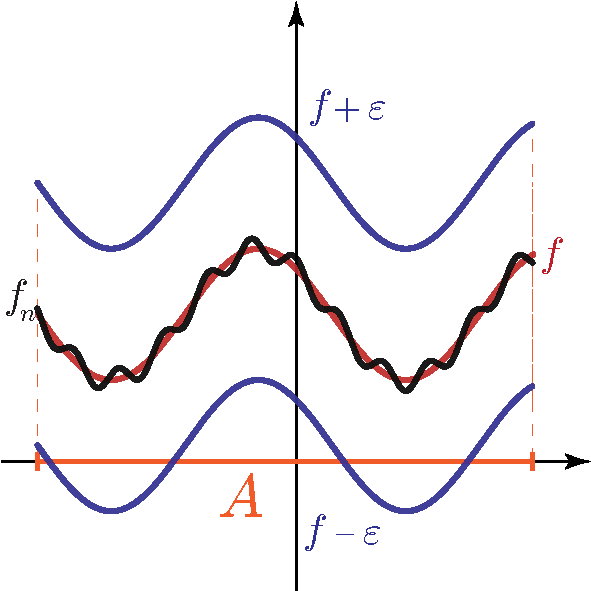
\includegraphics[trim=0cm 0cm 0cm 0cm, clip, scale=0.65]{images/visualizzazioneconvergenzauniforme.pdf}
\end{center}
\paragraph{Convergenza puntuale}
\begin{define}[Convergenza puntuale]
	Consideriamo l'insieme $X$ e le funzioni $\funz{f_n,f}{X}{\complexset}$.
	Si dice che $f_n$ \textbf{converge puntualmente}\index{convergenza!puntuale} a $f$\textbf{in} $X$ ($f_n\overset{\text{punt.}}{\to} f$) se
	\begin{equation}
		\forall x\in X,\lim_{n\to+\infty}f_n(x)=f(x)
	\end{equation}
	o, alternativamente,
	\begin{equation}
		\forall x\in X,\ \forall \epsilon >0,\ \exists N=N\left(x,\epsilon\right)\colon \forall n\geq N,\ \abs{f_n(x)-f(x)}<\epsilon
	\end{equation}
\end{define}
\begin{attention}
	Il limite della convergenza è in campo \textit{complesso}!
\end{attention}
\paragraph{Convergenza uniforme e puntuale}
Come visto in precedenza\footnote{Si veda \refChapterOnly{convergenzafunzioni}, sezione \ref{convuniformeimplicapuntuale}, pag. \pageref{convuniformeimplicapuntuale}.}, nella \textit{convergenza uniforme} il differente ordine dei quantificatori relativi alla $x$ fa sì che la soglia $N$ trovata è indipendente dal punto $x$ e quindi vale per ogni punto dell'insieme di definizione $X$, implicando pertanto la \textit{convergenza puntuale}.
\begin{multline}
	f_n\text{ converge uniformemente a }f\text{ su }X\implies\\
	\implies f_n\text{ converge puntualmente a }f\text{ in ogni punto di }X
\end{multline}
Il viceversa non è vero: abbiamo visto\footnote{Si veda nota precedente.} nella stessa sezione il caso della successione geometrica, la quale converge uniformemente solo a $f\equiv 0$ in ogni intervallo $\left[-a,a\right]\subsetneqq\left(-1,1\right),\ \forall a\in\left(0,1\right)$, mentre puntualmente in tutti i $\left(-1,1\right]$; qui di seguito riportiamo un controesempio alternativo.
\begin{example}\label{controesempiouniformepuntuale}
	Consideriamo la successione
	\begin{equation*}
		f_n(x)=\chi_{(n,n+1)}(x)=
		\begin{cases}
			\begin{array}{ll}
				1&n<x<n+1\\
				0&x\leq n\vee x\geq n+1
			\end{array}
		\end{cases}
	\end{equation*}
	Essa converge puntualmente a $f\equiv 0$:
	\begin{itemize}
		\item $\forall x\leq 0$ si ha che $f_n(x)\equiv 0,\ \forall n\in\naturalset$ e dunque banalmente $\displaystyle\lim_{n\to+\infty}f_n(x)=0$.
		\item $\forall x>0$, preso $N_x\coloneqq\floor{x}+1$ si ha che $\forall n>N_x\ f_n(x)=0$ e quindi $\displaystyle\lim_{n\to+\infty}f_n(x)=0$.
	\end{itemize}
	Tuttavia, essa non converge uniformemente a $0$ su $\realset$, dato che
	\begin{equation*}
		\lim_{n\to+\infty}\left(\sup_{x\in\realset}\abs{f_n(x)-f(x)}\right)=\lim_{n\to+\infty}\left(\sup_{x\in\realset}\abs{1-0}\right)=1\neq 0
	\end{equation*}
\end{example}
\paragraph{Convergenza quasi ovunque}
\begin{define}[Convergenza quasi ovunque]
	Consideriamo lo spazio di misura $\left(X,\mathcal{M},\mu\right)$ e le funzioni $\funz{f_n,f}{X}{\complexset}$ misurabili per ogni $n$. Si dice che
	$f_n$ \textbf{converge quasi ovunque}\index{convergenza!quasi ovunque} a $f$ \textbf{in} $X$ ($f_n\overset{\text{q.o.}}{\to} f$) se
	\begin{equation}
		\mu\left(\left\{x\in X \ \middle| \  \lim_{n\to+\infty}f_n(x)\neq f(x)\right\}\right)=0
	\end{equation}
\end{define}
\paragraph{Convergenza puntuale e quasi ovunque}
Dalla definizione è evidente che la convergenza \textit{quasi ovunque} nello spazio di misura $X$ è una \textit{convergenza puntuale} in $X$ tolto un insieme di misura nulla. Se in $\left(X,\mathcal{M},\mu\right)$ si ha convergenza puntuale, il sottoinsieme su cui \textit{non} vale è l'insieme vuoto e quindi è banalmente soddisfatta la condizione di convergenza \textbf{q.o.}, ossia
\begin{multline}
	f_n\text{ converge puntualmente a }f\text{ in ogni punto di }X\implies\\
	\implies f_n\text{ converge quasi ovunque a }f\text{ in ogni punto di }X
\end{multline}
Il viceversa non è vero, come possiamo vedere nel seguente esempio.
\begin{example}
	Consideriamo la successione
	\begin{equation*}
		f_n(x)=n\chi_{\left[0,\frac{1}{n}\right]}(x)=
		\begin{cases}
			\begin{array}{ll}
				n&0\leq x\leq\frac{1}{n}\\
				0&x< 0\vee x>\frac{1}{n}
			\end{array}
		\end{cases}
	\end{equation*}
	Osserviamo che la funzione non converge puntualmente a $f(x)=0$ su $\realset$:
	\begin{itemize}
		\item $\forall x< 0$ si ha che $f_n(x)\equiv 0,\ \forall n\in\naturalset$ e dunque banalmente $\displaystyle\lim_{n\to+\infty}f_n(x)=0$.
		\item $\forall x>0$, preso $N_x\coloneqq\frac{1}{x}$ si ha che $\forall n>N_x\ f_n(x)=0$ e quindi $\displaystyle\lim_{n\to+\infty}f_n(x)=0$.
		\item Per $x=0$ si ha $f_n(x)\equiv n,\ \forall n\in\naturalset$ e quindi $\displaystyle\lim_{n\to+\infty}f_n(x)=+\infty\neq0$.
	\end{itemize}
Tuttavia, l'insieme dove $f_n$ \textit{non} converge a $f\equiv0$ è un singolo punto e quindi ha misura nulla, pertanto $f_n$ converge \textbf{q.o.} a $f\equiv 0$.
\end{example}
\begin{observe}\label{indebolimentoteoremi}
	Possiamo indebolire le ipotesi del teorema della convergenza \textbf{monotona}\footnote{Si veda \refChapterOnly{integraledilebesgue}, teorema \ref{thmconvergenzamonotona}, pag. \pageref{thmconvergenzamonotona}.} e \textbf{dominata}\footnote{Si veda \refChapterOnly{integraledilebesgue}, teorema \ref{thmconvergenzadominata}, pag. \pageref{thmconvergenzadominata}.} per farli valere con delle ipotesi valide solo \textbf{q.o.}.
	\begin{itemize}
		\item Per la \textbf{convergenza monotona} è sufficiente anche solamente supporre che la successione $f_n$ sia non decrescente su $X$ tolto al più un insieme $N$ di misura nulla. In questo modo, la successione $f_n$ converge \textbf{q.o.} a $f$ su $X$ e vale il \textbf{passaggio al limite sotto segno di integrale}\index{passaggio al limite sotto segno di integrale} con la stessa dimostrazione di prima, in quanto
		\begin{equation*}
			\int_X f_nd\mu=\int_{X\setminus N}f_nd\mu\quad \text{e} \quad \int_X fd\mu=\int_{X\setminus N}fd\mu
		\end{equation*}
		Se la misura $\mu$ \textit{non} è completa, allora è necessario supporre che anche $f$ sia misurabile, a differenza del caso puntuale; se $\mu$ è invece completa, allora ciò non sarà necessario in quanto si può vedere che in tal caso una successione di funzioni misurabili converge \textbf{q.o.} ad una funzione misurabile\footnote{Nelle ‘‘Note aggiuntive'', a pag. \pageref{funzionimisurabiliqo} è possibile trovare la dimostrazione di questo risultato.} e dunque non è necessario aggiungere ipotesi.
		\item Per la \textbf{convergenza monotona} la convergenza della successione $f_n$ e la dominazione da parte di $g$ possono essere considerate proprietà valide \textbf{q.o.} purché la misura sia completa o la funzione limite $f$ è una funzione misurabile che coincide \textbf{q.o.} con il limite \textbf{q.o.} della successione, per lo stesso problema di misurabilità visto con la convergenza monotona  
	\end{itemize}
\end{observe}
\paragraph{Convergenza uniforme e quasi ovunque}
Dato che, come visto nel precedente controesempio, una successione di funzioni che converge \textbf{q.o.} su $X$ in generale non converge \textit{puntualmente} su $X$, oltremodo la convergenza \textbf{q.o.} non implica quella \textit{uniforme} su $X$.\\
Tuttavia, se \textit{restringiamo} opportunamente il dominio, è possibile trovare che una successione convergente \textbf{q.o.} converga anche \textit{uniformemente}, come afferma il seguente teorema.
\begin{theoremaqed}[Teorema di Egoroff]\index{teorema!di Egorofff}
	Consideriamo lo spazio di misura $\left(X,\mathcal{M},\mu\right)$ e le funzioni $\funz{f_n,f}{X}{\complexset}$.\\
	Supponiamo che esista $A\subseteq X$ con $\mu(A)<+\infty$, tale che $f_n$ converge \textbf{q.o.} a $f$ su $A$. Allora per ogni $\epsilon>0$ esiste un sottoinsieme misurabile $B\subseteq A$ tale che $\mu(B)< \epsilon$ e $f_n$ converge uniformemente a $f$ su $A\setminus B$.\\
	Equivalentemente, per ogni $\epsilon>0$ esiste un sottoinsieme misurabile $C\subseteq A$ tale che $\mu(A\setminus C)<\epsilon$  e $f_n$ converge uniformemente a $f$ su $C$.
\end{theoremaqed}
In altre parole, per qualunque successione $f_n$ convergente a $f$ \textbf{q.o} in $X$, se è possibile trovare un sottoinsieme $A\subseteq X$ misurabilmente finito allora $f_n$ converge anche uniformemente a $f$ in un qualunque sottoinsieme di $A$ con misura arbitrariamente vicina a quella originale. Una successione $f_n$ che converge a $f$ in questo modo è detta \textbf{convergenza quasi uniforme}\index{convergenza!quasi uniforme} - non utilizzeremo particolarmente questa nomenclatura.
L'ipotesi di $A$ con $\mu(A)<+\infty$ è fondamentale: infatti, possiamo riutilizzare come controesempio quello visto a pagina \pageref{controesempiouniformepuntuale} per la convergenza uniforme e puntuale.
\begin{example}
	Consideriamo la successione
	\begin{equation*}
		f_n(x)=\chi_{(n,n+1)}(x)=
		\begin{cases}
			\begin{array}{ll}
				1&n<x<n+1\\
				0&x\leq n\vee x\geq n+1
			\end{array}
		\end{cases}
	\end{equation*}
	Per quanto visto, essa converge puntualmente a $f\equiv 0$ su $\realset$ e quindi anche \textbf{q.o.}. Tuttavia, essa non converge uniformemente alla funzione nulla su qualunque sottoinsieme $\realset\setminus B$, per qualunque insieme $B$ di misura finita, dato che
	\begin{equation*}
		\lim_{n\to+\infty}\left(\sup_{x\in\realset\setminus B}\abs{f_n(x)-f(x)}\right)=\lim_{n\to+\infty}\left(\sup_{x\in\realset\setminus B}\abs{1-0}\right)=1\neq 0
	\end{equation*}
\end{example}
\paragraph{Convergenza in {$L^1$}}
\begin{define}[Convergenza in {$L^1\left(\mu\right)$}]
	Siano $f_n,f\in L^1\left(\mu\right)$. Si dice che
	$f_n$ \textbf{converge in $L^1\left(\mu\right)$}\index{convergenza!in $L^1\left(\mu\right)$} a $f$ ($f_n\overset{L^1}{\to} f$) se
	\begin{equation}
		\lim_{n\to+\infty}\norm{f_n-f}_1=\lim_{n\to+\infty}\int_{X}\abs{f_n-f}d\mu=0
	\end{equation}
\end{define}
Considerato $X\subseteq \realset$, possiamo visualizzare graficamente la convergenza in $L^1$.
\begin{center}
	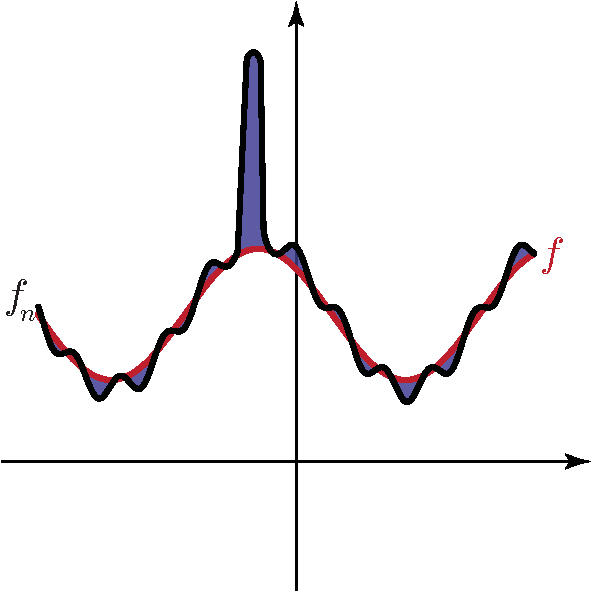
\includegraphics[trim=0cm 0cm 0cm 0cm, clip, scale=0.65]{images/visualizzazioneconvergenzal1.pdf}
\end{center}
Si nota che il grafico di $f_n$ può stare, in qualche zona, molto distante dal grafico di $f$, l'importante è che \textit{complessivamente} l'\textbf{area} tra $f_n$ e $f$ diminuisce, al crescere di $n$, fino ad essere \textit{nulla}.\\
Questa è la differenza principale tra la convergenza uniforme/puntuale/quasi ovunque e quella in $L^1$: se per le prime tre è fondamentale minimizzare la \textit{distanza} tra la funzione $f_n$ e $f$, l'ultima richiede di minimizzare l'\textit{area} tra le due.
\paragraph{Convergenza uniforme e in {$L^1$}}
\begin{theorema}[Legame tra convergenza uniforme e {$L^1$} nel caso di misura finita]
	Consideriamo lo spazio di misura $\left(X,\mathcal{M},\mu\right)$ e le funzioni $\funz{f_n,f}{X}{\complexset}$. Se
	\begin{enumerate}[label=(\alph*)]
		\item $f_n\in L^{1}\left(\mu\right)$.
		\item $f_n$ converge uniformemente a $f$ su $X$.
		\item $\mu(X)<+\infty$.
	\end{enumerate}
	allora
	\begin{enumerate}
		\item $f\in L^{1}\left(\mu\right)$.
		\item $\displaystyle\lim_{n\to+\infty}\norm{f_n-f}_1=0$.
		\item Vale il \textbf{passaggio al limite sotto segno di integrale}\index{passaggio al limite sotto segno di integrale}
		\begin{equation}
			\lim_{n\to+\infty}\int_Xf_nd\mu=\int_Xfd\mu
		\end{equation}
	\end{enumerate}
\end{theorema}
\begin{demonstration}~{}
	\begin{enumerate}[label=(\Roman*)]
		\item Dobbiamo dimostrare che $f\in L^!\left(\mu\right)$, ovvero
		\begin{itemize}
			\item $f$ misurabile.
			\item $\displaystyle\int_X\abs{f}d\mu<+\infty$
		\end{itemize}
		Per ipotesi si ha la convergenza uniforme di $f_n$ a $f$ in $X$:
		\begin{equation*}
			\circled[red]{\vardiamond}\quad \forall \epsilon > 0,\ \exists N=N\left(\epsilon\right)\colon \forall n\geq N,\ \abs{f_n(x)-f(x)}<\epsilon,\ \forall x\in X
		\end{equation*}
		Osserviamo che $f$ è dunque misurabile, in quanto la misurabilità passa al limite puntuale (e quindi al limite uniforme). Da $\circled[red]{\vardiamond}$ segue che
		\begin{equation*}
			\abs{f(x)}\underset{\forall n\in\naturalset}{=}\abs{f(x)-f_n(x)+f_n(x)}\leq\abs{f(x)-f_n(x)}+\abs{f_n(x)}\underset{\forall x\in X}{<}\epsilon +\abs{f(x)}
		\end{equation*}
		Posto, ad esempio, $\epsilon = 1$ e $n=N$ si ha
		\begin{equation*}
			\abs{f(x)}<1+\abs{f_N(x)},\ \forall x\in X
		\end{equation*}
		Allora
		\begin{align*}
			\int_X\abs{f}d\mu&\leq \int_X \left(1+\abs{f_N}\right)d\mu&\text{(monotonia integrale per l'integranda)}\\
			&=\int_{X}1d\mu+\int_X\abs{f_N}d\mu&\text{(additività dell'integranda)}\\
			&=\mu(X)+\int_X\abs{f_N}d\mu <+\infty&
		\end{align*}
		perché $\mu(x)<+\infty$ per ipotesi e $f_n\in L^1\left(\mu\right)$.
		\item Dobbiamo dimostrare che $\displaystyle\lim_{n\to+\infty}\norm{f_n-f}_1=0$, ossia
		\begin{equation*}
			\circled[blue]{\spadesuit}\quad \forall \epsilon > 0,\ \exists \widetilde{N}=\widetilde{N}\left(\epsilon\right)\colon \forall n\geq N,\ \norm{f_n(x)-f(x)}_1<\epsilon
		\end{equation*}
		Si ha
		\begin{equation*}
			\norm{f_n-f}_1=\int_X\abs{f_n-f}d\mu\underset{\forall n\geq N\left(\epsilon\right)}{\overset{\circled[red]{\vardiamond}}{\leq}}\int_X\epsilon d\mu=\epsilon \mu(X)<+\infty
		\end{equation*}
		Vale la relazione \circled[blue]{\spadesuit} ponendo $\widetilde{N}=N$.
		\item Segue dal punto $II$ come nell'ultima parte della dimostrazione del \textit{teorema di convergenza dominata}.
	\end{enumerate}
\end{demonstration}
\begin{attention}
	Se $\mu(X)=+\infty$, in generale \textit{non} vale nessuna delle tesi: come controesempi si possono prendere i tre esposti\footnote{Si veda \refChapterOnly{convergenzafunzioni}, pag. \pageref{controesempipassaggiointegrale}.} nel discorso sui problemi di integrabilità nell'ambito della teoria di Riemann.
\end{attention}
In generale non vale il viceversa: dalla convergenza in $L^1$ non segue quella uniforme.
\begin{examplewt}[Convergenza in $L^1$ non implica convergenza uniforme.]
	Consideriamo la successione
	\begin{equation*}
		f_n(x)=n\chi_{\left[0,\frac{1}{n^2}\right]}(x)=
		\begin{cases}
			\begin{array}{ll}
				n&0\leq x\leq\frac{1}{n^2}\\
				0&x< 0\vee x>\frac{1}{n^2}
			\end{array}
		\end{cases}
	\end{equation*}
	La successione converge in $L^1$ a $f\equiv 0$:
	\begin{equation*}
		\lim_{n\to+\infty}\norm{f_n-f}_1=\lim_{n\to+\infty}\int_{\realset}\abs{f_n-f}d\mu=\lim_{n\to+\infty}\int_{0}^{\frac{1}{n^2}}ndx=\lim_{n\to+\infty}n\cdot\frac{1}{n^2}=\lim_{n\to+\infty}\frac{1}{n}=0
	\end{equation*}
	Tuttavia, essa non converge uniformemente a $0$ su $\realset$, dato che
	\begin{equation*}
		\lim_{n\to+\infty}\left(\sup_{x\in\realset}\abs{f_n(x)-f(x)}\right)=\lim_{n\to+\infty}\left(\sup_{x\in\realset}\abs{n-0}\right)=+\infty\neq 0
	\end{equation*}
\end{examplewt}
\begin{observe}
	Questo teorema ci mostra che il passaggio al limite sotto segno di integrale visto nell'ambito della teoria di Riemann, che contemplava la convergenza uniforme su intervalli limitati, è valido anche nell'ambito della Teoria di Lebesgue.
\end{observe}
Con questo teorema abbiamo finalmente risposto in toto ad uno dei quesiti inizialmente enunciati nel \refChapterOnly{ellipseintroduction}: nell'ambito della teoria di Lebesgue, ci sono tre differenti teoremi per il passaggio al limite sotto il segno di integrale, che sono quelli di
\begin{itemize}
	\item Convergenza uniforme su spazi di misura finita.
	\item Convergenza monotona.
	\item Convergenza dominata.
\end{itemize}
Esistono anche degli analoghi per lo scambio di serie ed integrale.
\paragraph{Convergenza quasi ovunque e {$L^1$}}
Come abbiamo detto precedentemente\footnote{Si veda pag. \pageref{indebolimentoteoremi}.} possiamo indebolire le ipotesi dei teoremi di convergenza monotona e dominata per applicarli anche alla convergenza \textbf{q.o.}, e tutti e due implicano il passaggio al limite sotto segno di integrale. Questo ci permette di affermare il seguente corollario.
\begin{corollaryqed}[Convergenza quasi ovunque e {$L^1$}]
	Consideriamo lo spazio di misura $\left(X,\mathcal{M},\mu\right)$ e le funzioni $\funz{f_n,f}{X}{\complexset}$ misurabili; inoltre, sia $f_n$ convergente \textbf{q.o.} a $f$ e tale per cui sia soddisfatta almeno una delle seguenti:
	\begin{itemize}
		 \item Valgono le ipotesi del teorema di convergenza \textit{monotona} - in particolare, la successione è crescente positiva.
		 \item Valgono le ipotesi del teorema di convergenza \textit{dominata} - in particolare, la successione ha una dominazione uniforme e integrabile.
	\end{itemize}
	Se valgono queste condizioni, allora $f_n$ converge in $L^1$ a $f$.
\end{corollaryqed}
Chiaramente, questo corollario è valido anche per successioni che convergono \textit{puntualmente} ad una funzione limite e che soddisfano le ipotesi di uno dei due teoremi.\\
Purtroppo, dalla convergenza in $L^1$ a quella \textbf{q.o.} in generale non si può dire nulla, come si può vedere da un controesempio dal nome peculiare.
\begin{examplewt}[Successione della macchina da scrivere]
		Consideriamo la successione
	\begin{equation*}
		f_n(x)=\chi_{\left[\frac{n-2^k}{2^k},\frac{n-2^k+1}{2^k}\right]}(x)=
		\begin{cases}
			\begin{array}{ll}
				1&\frac{n-2^k}{2^k}\leq x\leq\frac{n-2^k+1}{2^k}\\
				0&x< \frac{n-2^k}{2^k}\vee x>\frac{n-2^k+1}{2^k}
			\end{array}
		\end{cases}
	\end{equation*}
	per ogni $n\geq 0$ e con $k\in\naturalset$ tale che $2^k\leq n\leq 2^{k+1}$. Questa si può visualizzare come dei segmenti, ad altezza $1$ e larghezza $\frac{1}{2^k}$, che ‘‘marciano'' lungo l'intervallo $\left[0,1\right]$ ripetutamente. Ad ogni ‘‘ritorno a capo'' la larghezza viene dimezzata.\\
	Si vede che $f_n$ converge alla funzione $f\equiv 0$ in $L^1$: il segmento individuato da $f_n$ tenderà a diventare un singolo punto al crescere di $n$, dunque l'area sottesa da $f_n$ è un segmento verticale ed è quindi di misura nulla; infatti,
	\begin{align*}
		\lim_{n\to+\infty}\norm{f_n-f}_1&=\lim_{n\to+\infty}\int_{\realset}\abs{f_n-f}d\mu = \lim_{n\to+\infty}\int_{\frac{n-2^k}{2^k}}^{\frac{n-2^k+1}{2^k}}!dx = \\
		& = \lim_{n\to+\infty}\left(\frac{n-2^k+1}{2^k}-\frac{n-2^k}{2^k}\right) = \lim_{n\to+\infty}\frac{1}{2^k}=0
	\end{align*}
	Invece, $f_n$ non converge \textbf{q.o.} a $f\equiv 0$. Infatti, per qualunque scelta di $x\in\left[0,1\right]$ e per qualunque $N\in\naturalset$ si può trovare un $n>N$ con $f_n(x)=1$, quindi la sequenza non può convergere \textit{mai} a $0$.
\end{examplewt}
Tuttavia, se consideriamo delle \textit{sottosuccessioni}, allora è sempre possibile trovare una sottosuccessione convergente \textbf{q.o.}.
\begin{theoremaqed}[Teorema della convergenza dominata inversa]
	Sia $\left(X,\mathcal{M},\mu\right)$ uno spazio di misura e $\funz{f_n}{X}{\complexset}$, con $f_n\in L^1(\mu),\ \forall n$, una successione di funzioni tale che $f_n$ converge ad una funzione $f$ in $L^1$. Allora esiste una sottosuccessione $f_{n_k}$ e una funzione $g\in L^1(\mu)$ tale che
	\begin{enumerate}
		\item $f_{n_k}$ converge a $f$ \textbf{q.o.} - rispetto a $k$.
		\item $\forall k\in\naturalset,\abs{f_{n_k}(x)}\leq g(x)$ \textbf{q.o.} per ogni $x\in X$.\qedhere
	\end{enumerate} 
\end{theoremaqed}
\paragraph{Convergenza in misura}
\begin{define}[Convergenza in misura]
	Consideriamo lo spazio di misura $\left(X,\mathcal{M},\mu\right)$ e le funzioni $\funz{f_n,f}{X}{\complexset}$ misurabili per ogni $n$; $\forall n\in\naturalset$ definiamo la funzione $g_n\coloneqq \abs{f_n-f}$. Allora, se prendiamo $\forall n\in\ \naturalset,\forall \epsilon>0$ l'insieme
	\begin{equation*}
		E_{n,\epsilon}\coloneqq g^{-1}_n\left(\left(\epsilon,+\infty\right)\right)\footnote{Siccome $f_n, f$ sono misurabili, allora anche $g$ lo è. Inoltre siccome $(\epsilon,+\infty)$ è un aperto allora $g^{-1}_n\left(\left(\epsilon,+\infty\right)\right)\in\mathcal{M},\ \forall\epsilon >0,\ \forall n$.}
		=\left\{x\in X\mid \abs{f_n(x)-f(x)}>\epsilon\right\}
	\end{equation*}
	si dice che	$f_n$ \textbf{converge in misura}\index{convergenza!in misura} a $f$ ($f_n\overset{\mu}{\to} f$) se
	\begin{equation}
		\lim_{n\to+\infty}\mu\left(\left\{x\in X\mid \abs{f_n(x)-f(x)}>\epsilon\right\}\right)=0,\ \forall \epsilon >0
	\end{equation}
\end{define}
Considerato $X\subseteq \realset$, possiamo visualizzare graficamente la convergenza in misura.
\begin{center}
	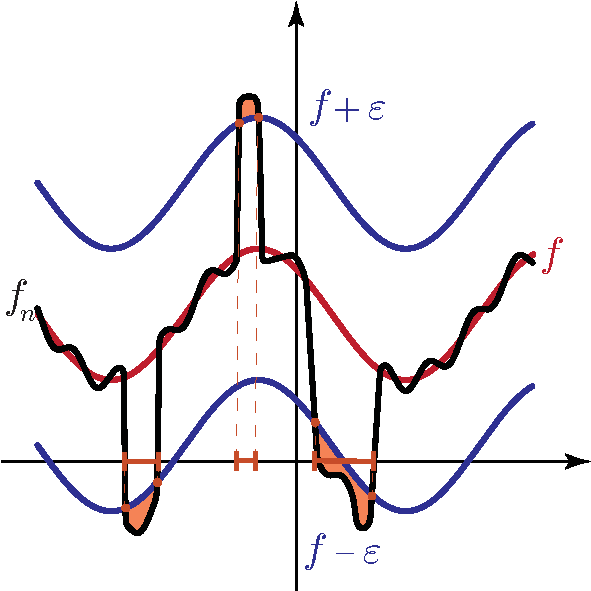
\includegraphics[trim=0cm 0cm 0cm 0cm, clip, scale=0.55]{images/visualizzazioneconvergenzamisura.pdf}
\end{center}
Possiamo interpretare questa convergenza come un particolare tipo di convergenza in $L^1$, condividendo però alcune caratteristiche con la convergenza \textit{uniforme} e alla convergenza \textit{quasi ovunque}. Arbitrariamente scelto un raggio $\epsilon$, il grafico di $f_n$ è nella quasi sua totalità contenuto nell'\textit{intorno tubulare} di raggio $\epsilon$ centrato sul grafico di $f$, ma è concesso che esso possa \textit{uscire} da tale intorno purché la misura dell'insieme di tutti i punti di $\realset$ in cui ciò accade tenda ad essere nulla al crescere di $n$.
\paragraph{Convergenza in {$L^1$} e in misura}
\begin{theorema}[Legame tra convergenza {$L^1$} e convergenza in misura]
	Consideriamo lo spazio di misura $\left(X,\mathcal{M},\mu\right)$ e le funzioni $\funz{f_n,f}{X}{\complexset}$ tali che $f_n,f\in L^1\left(\mu\right)$.
	Allora
	\begin{equation}
		f_n\text{ converge in }L^1\text{ a }f\implies f_n\text{ converge in misura a }f
	\end{equation}
\end{theorema}
\begin{demonstration}
	Dobbiamo dimostrare che
	\begin{equation*}
		\mu\bigg(\underbrace{\left\{x\in X\ \middle| \ \abs{f_n(x)-f(x)}>\epsilon\right\}}_{\coloneqq E_{n,\epsilon}}\bigg)=0,\ \forall \epsilon>0
	\end{equation*}
	Si ha, per monotonia dell'integrale rispetto al dominio,
	\begin{equation*}
		\int_X\abs{f_n-f}d\mu\geq\int_{E_{n,\epsilon}}\abs{f_n-f}d\mu\geq\epsilon\int_{E_{n,\epsilon}}d\mu=\epsilon\mu\left(E_{n.,\epsilon}\right),\ \forall \epsilon>0,\ \forall n\geq 1
	\end{equation*}
	Dunque si ottiene
	\begin{equation*}
		0\leq \mu\left(E_{n,\epsilon}\right)\leq \frac{1}{\epsilon}\int_X\abs{f_n-f}d\mu=\frac{1}{\epsilon}\underbrace{\norm{f_n-f}_1}_{\substack{\to 0\text{ per }\\n\to+\infty}}
	\end{equation*}
	Passando al limite per $n\to+\infty$, applicando il \textit{teorema del confronto} si ricava:
	\begin{equation*}
		\lim_{n\to+\infty}\mu\left(E_{n,\epsilon}\right)=0,\ \forall \epsilon>0\qedhere
	\end{equation*}
\end{demonstration}
In generale, non vale il viceversa: una successione che converge in misura non necessariamente converge in $L^1$.
\begin{example}
	Consideriamo la successione
	\begin{equation*}
		f_n(x)=n\chi_{\left[0,\frac{1}{n}\right]}(x)=
		\begin{cases}
			\begin{array}{ll}
				n&0\leq x\leq\frac{1}{n}\\
				0&x< 0\vee x>\frac{1}{n}
			\end{array}
		\end{cases}
	\end{equation*}
	La successione \textit{non} converge in $L^1$ a $f\equiv 0$:
	\begin{equation*}
		\lim_{n\to+\infty}\norm{f_n-f}_1=\lim_{n\to+\infty}\int_{\realset}\abs{f_n-f}d\mu=\lim_{n\to+\infty}\int_{0}^{\frac{1}{n}}ndx=\lim_{n\to+\infty}n\cdot\frac{1}{n}=\lim_{n\to+\infty}1=1\neq 0
	\end{equation*}
	Tuttavia, essa converge in misura a $0$ su $\realset$, dato che
	\begin{align*}
		&\left\{x\in X\mid \abs{f_n(x)-f(x)}>\epsilon\right\}=\left\{x\in X\mid \abs{f_n(x)}>\epsilon\right\}=\left[0,n\right],\ \forall \epsilon>0\\
		&\implies\lim_{n\to+\infty}\mu\left(\left\{x\in X\mid \abs{f_n(x)-f(x)}>\epsilon\right\}\right)=\lim_{n\to+\infty}\mu\left(\left[0,\frac{1}{n}\right]\right)=\lim_{n\to+\infty}\frac{1}{n}=0,\ \forall \epsilon >0
	\end{align*}
\end{example}
\paragraph{Convergenza quasi ovunque e in misura}
\begin{theoremaqed}[Legame tra convergenza quasi ovunque e in misura]
	Consideriamo lo spazio di misura $\left(X,\mathcal{M},\mu\right)$ e le funzioni $\funz{f_n,f}{X}{\complexset}$.
	\begin{enumerate}
		\item Se $\mu(X)<+\infty$ e $f_n$ converge \textbf{q.o.} a $f$ su $X$, allora $f_n$ converge in misura a $f$ su $X$.
		\item Se $\mu$ è $\sigma$-finita e $f_n$ converge in misura a $f$ su $X$, allora c'è una sottosuccessione $f_{n_k}$ convergenza \textbf{q.o.} a $f$ su $X$.\qedhere
	\end{enumerate}
\end{theoremaqed}
Chiaramente, il secondo punto del teorema è valido - nelle ipotesi del teorema - anche per successioni che convergono in $L^1$, dato che convergono sempre anche in misura.